% CS631D Advanced Programming in the UNIX Environment
% Author: Jan Schaumann <jschauma@netmeister.org>
% $Id: slides.tex,v 1.6 2004/07/16 01:56:50 jschauma Exp $
\special{! TeXDict begin /landplus90{true}store end }

\documentclass[xga]{xdvislides}
\usepackage[landscape]{geometry}
\usepackage{graphics}
\usepackage{graphicx}
\usepackage{colordvi}

\begin{document}
\setfontphv

%%% Headers and footers
\lhead{\slidetitle}
\chead{CS631 - Advanced Programming in the UNIX Environment}
\rhead{\relax}
\lfoot{\Gray{Lecture 02: File I/O, File Sharing}}
\cfoot{\relax}
\rfoot{\Gray{\today}}

\vspace*{\fill}
\begin{center}
	\Hugesize
		CS631 - Advanced Programming in the UNIX Environment\\ [1em]
		File I/O, File Sharing
	\hspace*{5mm}\blueline\\ [1em]
	\Normalsize
		Department of Computer Science\\
		Stevens Institute of Technology\\
		Jan Schaumann\\
		\verb+jschauma@stevens.edu+\\
		\verb+http://www.cs.stevens.edu/~jschauma/631/+
\end{center}
\vspace*{\fill}

\subsection{File Descriptors}
\begin{itemize}
	\item A {\em file descriptor} (or {\em file handle}) is a small,
		non-negative integer which identifies a file to the kernel.
\end{itemize}


\subsection{File Descriptors}
\begin{itemize}
	\item A {\em file descriptor} (or {\em file handle}) is a small,
		non-negative integer which identifies a file to the kernel.
	\item Traditionally, {\tt stdin}, {\tt stdout} and {\tt stderr}
		are 0, 1 and 2 respectively.
\end{itemize}

\subsection{File Descriptors}
\begin{itemize}
	\item A {\em file descriptor} (or {\em file handle}) is a small,
		non-negative integer which identifies a file to the kernel.
	\item Traditionally, {\tt stdin}, {\tt stdout} and {\tt stderr}
		are 0, 1 and 2 respectively.
\end{itemize}
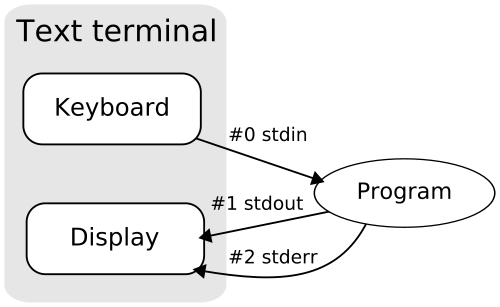
\includegraphics[scale=0.6,angle=-90]{pics/stdstreams.eps}

\subsection{File Descriptors}
\begin{itemize}
	\item A {\em file descriptor} (or {\em file handle}) is a small,
		non-negative integer which identifies a file to the kernel.
	\item Traditionally, {\tt stdin}, {\tt stdout} and {\tt stderr}
		are 0, 1 and 2 respectively.
\end{itemize}
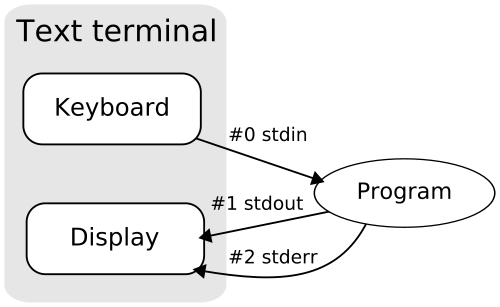
\includegraphics[scale=0.61,angle=-90]{pics/stdstreams.eps}
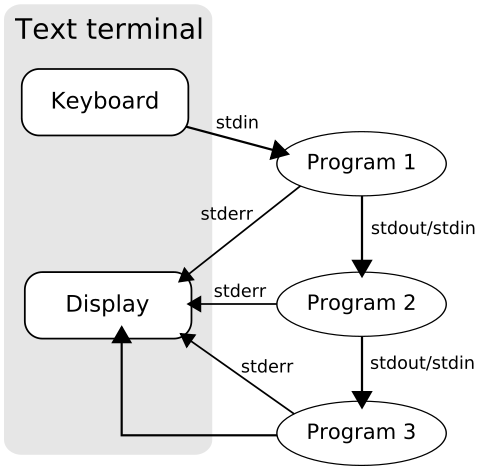
\includegraphics[scale=0.53,angle=-90]{pics/pipeline.eps}



\subsection{File Descriptors}
\begin{itemize}
	\item A {\em file descriptor} (or {\em file handle}) is a small,
		non-negative integer which identifies a file to the kernel.
	\item Traditionally, {\tt stdin}, {\tt stdout} and {\tt stderr}
		are 0, 1 and 2 respectively.
	\item Relying on ``magic numbers'' is Bad\texttrademark.  Use {\tt
		STDIN\_FILENO}, {\tt STDOUT\_FILENO} and {\tt STDERR\_FILENO}.
\end{itemize}

\subsection{File Descriptors}
\begin{itemize}
	\item A {\em file descriptor} (or {\em file handle}) is a small,
		non-negative integer which identifies a file to the kernel.
	\item Traditionally, {\tt stdin}, {\tt stdout} and {\tt stderr}
		are 0, 1 and 2 respectively.
	\item Relying on ``magic numbers'' is Bad\texttrademark.  Use {\tt
		STDIN\_FILENO}, {\tt STDOUT\_FILENO} and {\tt STDERR\_FILENO}.
\end{itemize}

\addvspace{.5in}
\begin{center}
\Huge
\verb+openmax.c+
\normalsize
\end{center}

\vspace*{\fill}
See also: \verb+http://en.wikipedia.org/wiki/File_descriptor+

\subsection{Standard I/O}
Basic File I/O: almost all UNIX file I/O can be
performed using these five functions:
\begin{itemize}
	\item {\tt open(2)}
	\item {\tt close(2)}
	\item {\tt lseek(2)}
	\item {\tt read(2)}
	\item {\tt write(2)}
\end{itemize}
\vspace{.25in}
Processes may want to share recources.  This requires us to look at:
\begin{itemize}
	\item atomicity of these operations
	\item file sharing
	\item manipulation of file descriptors
\end{itemize}

\subsection{{\tt creat(2)}}
\small
\setlength{\unitlength}{1mm}
\begin{center}
	\begin{picture}(200,25)
		\thinlines
		\put(0,0){\framebox(180,25){}}
		\put(10,20){{\tt \#include <fcntl.h>}}
		\put(10,10){{\tt int creat(const char *{\em pathname}, mode\_t {\em mode});}}
		\put(115,3){Returns:  file descriptor if OK, -1 on error}
	\end{picture}
\end{center}
\begin{center}
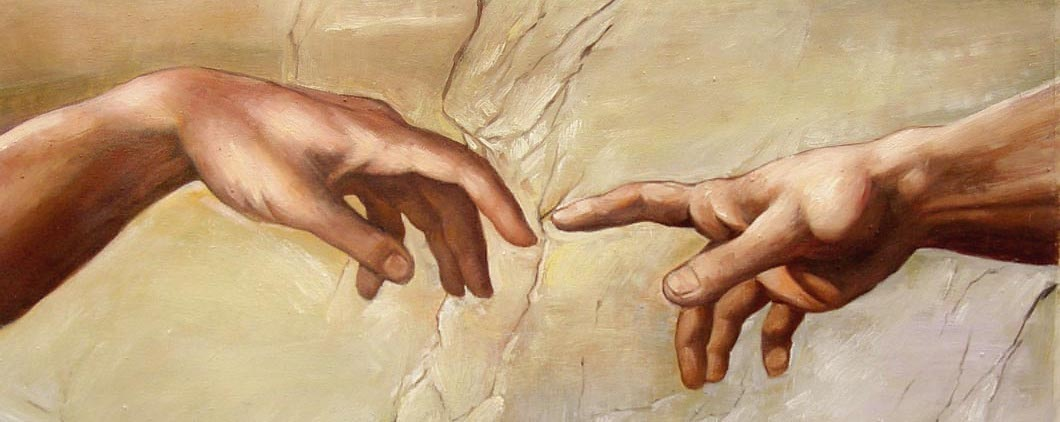
\includegraphics[scale=0.8,angle=-90]{pics/creation.eps} \\
\small
\verb+http://is.gd/x4KPa2+
\end{center}
\Normalsize

\subsection{{\tt creat(2)}}
\small
\setlength{\unitlength}{1mm}
\begin{center}
	\begin{picture}(200,25)
		\thinlines
		\put(0,0){\framebox(180,25){}}
		\put(10,20){{\tt \#include <fcntl.h>}}
		\put(10,10){{\tt int creat(const char *{\em pathname}, mode\_t {\em mode});}}
		\put(115,3){Returns:  file descriptor if OK, -1 on error}
	\end{picture}
\end{center}
\Normalsize
\vspace{.5in}
{\bf This interface is made obsolete by {\tt open(2)}.} \\

\subsection{{\tt open(2)}}
\small
\setlength{\unitlength}{1mm}
\begin{center}
	\begin{picture}(200,25)
		\thinlines
		\put(0,0){\framebox(180,25){}}
		\put(10,20){{\tt \#include <fcntl.h>}}
		\put(10,12){{\tt int open(const char *{\em pathname}, int {\em oflag}, ... /* mode\_t {\em mode} */ );}}
		\put(115,3){Returns:  file descriptor if OK, -1 on error}
	\end{picture}
\end{center}
\vspace{.25in}
\Normalsize
{\em oflag} must be one (and only one) of:
\small
\begin{itemize}
	\item {\tt O\_RDONLY} -- Open for reading only
	\item {\tt O\_WRONLY} -- Open for writing only
	\item {\tt O\_RDWR} -- Open for reading and writing
\end{itemize}
\vspace{.25in}
\Normalsize
and may be OR'd with any of these:
\small
\begin{itemize}
	\item {\tt O\_APPEND} -- Append to end of file for each write
	\item {\tt O\_CREAT} -- Create the file if it doesn't exist. Requires
		{\em mode} argument
	\item {\tt O\_EXCL} -- Generate error if {\tt O\_CREAT} and file
		already exists. (atomic)
	\item {\tt O\_TRUNC} -- If file exists and successfully open in
		{\tt O\_WRONLY} or {\tt O\_RDWR}, make length = 0
	\item {\tt O\_NOCTTY} -- If pathname refers to a terminal device, do
		not allocate the device as a controlling terminal
	\item {\tt O\_NONBLOCK} -- If pathname refers to a FIFO, block special,
		or char special, set nonblocking mode (open and I/O)
	\item {\tt O\_SYNC} --  Each write waits for physical I/O to complete
\end{itemize}

\subsection{{\tt close(2)}}
\small
\setlength{\unitlength}{1mm}
\begin{center}
	\begin{picture}(200,25)
		\thinlines
		\put(0,0){\framebox(180,25){}}
		\put(10,20){{\tt \#include <unistd.h>}}
		\put(10,10){{\tt int close(int {\em fd});}}
		\put(115,3){Returns:  0 if OK, -1 on error}
	\end{picture}
\end{center}
\Normalsize
\vspace{.25in}
\begin{itemize}
	\item closing a filedescriptor releases any record locks on
		that file (more on that in future lectures)
	\item file descriptors not explicitly closed are closed by the kernel
		when the process terminates.
\end{itemize}

\subsection{{\tt read(2)}}
\small
\setlength{\unitlength}{1mm}
\begin{center}
	\begin{picture}(200,25)
		\thinlines
		\put(0,0){\framebox(180,25){}}
		\put(10,20){{\tt \#include <unistd.h>}}
		\put(10,12){{\tt ssize\_t read(int {\em filedes}, void *{\em buff}, size\_t {\em nbytes} );}}
		\put(85,3){Returns:  number of bytes read, 0 if end of file, -1 on error}
	\end{picture}
\end{center}
\Normalsize
\begin{center}

\includegraphics[scale=0.4,angle=-90]{pics/reading.eps} \\
\small
\verb+http://is.gd/qI5r8E+
\end{center}
\Normalsize


\subsection{{\tt read(2)}}
\small
\setlength{\unitlength}{1mm}
\begin{center}
	\begin{picture}(200,25)
		\thinlines
		\put(0,0){\framebox(180,25){}}
		\put(10,20){{\tt \#include <unistd.h>}}
		\put(10,12){{\tt ssize\_t read(int {\em filedes}, void *{\em buff}, size\_t {\em nbytes} );}}
		\put(85,3){Returns:  number of bytes read, 0 if end of file, -1 on error}
	\end{picture}
\end{center}
\Normalsize
There can be several cases where {\tt read} returns less than the number of
bytes requested:
\begin{itemize}
	\item EOF reached before requested number of bytes have been read
    \item Reading from a terminal device, one "line" read at a time
    \item Reading from a network, buffering can cause delays in arrival of data
    \item Record-oriented devices (magtape) may return data one record at
		a time
\end{itemize}
\vspace{.25in}
{\tt read} begins reading at the current offset, and increments the offset
by the number of bytes actually read.
% Note that {\tt ssize\_t} is a signed
% type, while {\tt size\_t} is unsigned.

\subsection{{\tt write(2)}}
\small
\setlength{\unitlength}{1mm}
\begin{center}
	\begin{picture}(200,25)
		\thinlines
		\put(0,0){\framebox(180,25){}}
		\put(10,20){{\tt \#include <unistd.h>}}
		\put(10,12){{\tt ssize\_t write(int {\em filedes}, void *{\em buff}, size\_t {\em nbytes} );}}
		\put(85,3){Returns:  number of bytes written if OK, -1 on error}
	\end{picture}
\end{center}
\Normalsize
\vspace{.25in}
\begin{itemize}
	\item {\tt write} returns {\tt nbytes} or an error has occurred (disk
		full, file size limit exceeded, ...)
	\item for regular files, {\tt write} begins writing at the
		current offset (unless {\tt O\_APPEND} has been specified, in which
		case the offset is first set to the end of the file)
	\item after the write, the offset is
		adjusted by the number of bytes actually written
\end{itemize}

\subsection{{\tt lseek(2)}}
\small
\setlength{\unitlength}{1mm}
\begin{center}
	\begin{picture}(200,30)
		\thinlines
		\put(0,0){\framebox(180,30){}}
		\put(10,25){{\tt \#include <sys/types.h>}}
		\put(10,20){{\tt \#include <fcntl.h>}}
		\put(10,12){{\tt off\_t lseek(int {\em filedes}, off\_t {\em offset}, int {\em whence} );}}
		\put(115,3){Returns:  new file offset if OK, -1 on error}
	\end{picture}
\end{center}
\Normalsize
\begin{center}
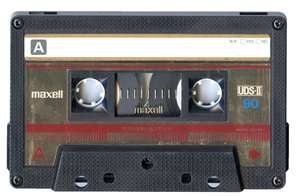
\includegraphics[scale=0.9,angle=-90]{pics/tape.eps} \\
\small
\verb+http://is.gd/3fp5Vx+
\end{center}
\Normalsize


\subsection{{\tt lseek(2)}}
\small
\setlength{\unitlength}{1mm}
\begin{center}
	\begin{picture}(200,30)
		\thinlines
		\put(0,0){\framebox(180,30){}}
		\put(10,25){{\tt \#include <sys/types.h>}}
		\put(10,20){{\tt \#include <fcntl.h>}}
		\put(10,12){{\tt off\_t lseek(int {\em filedes}, off\_t {\em offset}, int {\em whence} );}}
		\put(115,3){Returns:  new file offset if OK, -1 on error}
	\end{picture}
\end{center}
\Normalsize
\vspace{.25in}
The value of whence determines how offset is used:
\small
\begin{itemize}
	\item {\tt SEEK\_SET} bytes from the beginning of the file
	\item {\tt SEEK\_CUR} bytes from the current file position
	\item {\tt SEEK\_END} bytes from the end of the file
\end{itemize}
\Normalsize
\vspace{.25in}
``Weird'' things you can do using {\tt lseek(2)}:
\begin{itemize}
	\item seek to a negative offset
	\item seek 0 bytes from the current position
	\item seek past the end of the file
\end{itemize}

\subsection{{\tt lseek(2)}}
\begin{verbatim}
$ cc -Wall lseek.c
$ ./a.out < lseek.c
seek OK
$ cat lseek.c | ./a.out
cannot seek
$ mkfifo fifo
$ ./a.out <fifo

\end{verbatim}



\subsection{{\tt lseek(2)}}
\begin{verbatim}
$ cc -Wall hole.c
$ ./a.out
$ ls -l file.hole
-rw-------  1 jschauma  wheel  10240020 Sep 18 17:20 file.hole
$ hexdump -c file.hole
0000000   a   b   c   d   e   f   g   h   i   j  \0  \0  \0  \0  \0  \0
0000010  \0  \0  \0  \0  \0  \0  \0  \0  \0  \0  \0  \0  \0  \0  \0  \0
*
09c4000  \0  \0  \0  \0  \0  \0  \0  \0  \0  \0   A   B   C   D   E   F
09c4010   G   H   I   J
09c4014
$ cat file.hole > file.nohole
$ ls -ls file.*
   96 -rw-------  1 jschauma  wheel  10240020 Sep 18 17:20 file.hole
20064 -rw-r--r--  1 jschauma  wheel  10240020 Sep 18 17:21 file.nohole
\end{verbatim}

See also: \verb+http://en.wikipedia.org/wiki/Sparse_file+ (not on HFS+)


\subsection{{\tt I/O Efficiency}}
Caveats with the program {\tt simple-cat.c} from the last class:
\begin{itemize}
	\item assumes that {\em stdin} and {\em stdout} have been set up
		appropriately
\end{itemize}

\subsection{{\tt I/O Efficiency}}
Caveats with the program {\tt simple-cat.c} from the last class:
\begin{itemize}
	\item assumes that {\em stdin} and {\em stdout} have been set up
		appropriately
	\item works for ``text'' and ``binary'' files since there is no such
		distinction in the UNIX kernel
\end{itemize}

\subsection{{\tt I/O Efficiency}}
Caveats with the program {\tt simple-cat.c} from the last class:
\begin{itemize}
	\item assumes that {\em stdin} and {\em stdout} have been set up
		appropriately
	\item works for ``text'' and ``binary'' files since there is no such
		distinction in the UNIX kernel
	\item how do we know the optimal {\tt BUFFSIZE}?
\end{itemize}

\subsection{{\tt I/O Efficiency}}
\begin{verbatim}
$ for n in $(seq 10); do
dd if=/dev/urandom of=file$n count=20480
done
$ i=1
$ for n in 1 512 1024 2048 4096 8192 16384 32768 65536 131072; do
cc -Wall -DBUFFSIZE=$n simple-cat.c
time ./a.out <file$i > file$i.copy
i=$(( $i + 1 ))
done

\end{verbatim}

Note: results vary depending on OS/filesystem.

\subsection{File Sharing}
Since UNIX is a multi-user/multi-tasking system, it is conceivable (and
useful) if more than one process can act on a single file simultaneously. In
order to understand how this is accomplished, we need to examine some kernel
data structures which relate to files.  (See: Stevens, pp 70 ff)

\subsection{File Sharing}
Since UNIX is a multi-user/multi-tasking system, it is conceivable (and
useful) if more than one process can act on a single file simultaneously. In
order to understand how this is accomplished, we need to examine some kernel
data structures which relate to files.  (See: Stevens, pp 70 ff)

\begin{itemize}
	\item each process table entry has a table of file descriptors, which contain
		\begin{itemize}
			\item the file descriptor flags (\verb+fcntl(2)+)
			\item a pointer to a file table entry
		\end{itemize}
\end{itemize}

\subsection{File Sharing}
Since UNIX is a multi-user/multi-tasking system, it is conceivable (and
useful) if more than one process can act on a single file simultaneously. In
order to understand how this is accomplished, we need to examine some kernel
data structures which relate to files.  (See: Stevens, pp 70 ff)

\begin{itemize}
	\item each process table entry has a table of file descriptors, which contain
		\begin{itemize}
			\item the file descriptor flags (\verb+fcntl(2)+)
			\item a pointer to a file table entry
		\end{itemize}
	\item the kernel maintains a file table;  each entry contains
		\begin{itemize}
			\item file status flags (\verb+O_APPEND+, \verb+O_SYNC+, \verb+O_RDONLY+, etc.)
			\item current offset
			\item pointer to a vnode table entry
		\end{itemize}
\end{itemize}

\subsection{File Sharing}
Since UNIX is a multi-user/multi-tasking system, it is conceivable (and useful)
if more than one process can act on a single file simultaneously. In
order to understand how this is accomplished, we need to examine some kernel
data structures which relate to files.  (See: Stevens, pp 70 ff)

\begin{itemize}
	\item each process table entry has a table of file descriptors, which
		contain
		\begin{itemize}
			\item the file descriptor flags (\verb+fcntl(2)+)
			\item a pointer to a file table entry
		\end{itemize}
	\item the kernel maintains a file table;  each entry contains
		\begin{itemize}
			\item file status flags (\verb+O_APPEND+, \verb+O_SYNC+, \verb+O_RDONLY+, etc.)
			\item current offset
			\item pointer to a vnode table entry
		\end{itemize}
	\item a vnode structure contains
		\begin{itemize}
			\item vnode information
			\item inode information (such as current file size)
		\end{itemize}
\end{itemize}

\subsection{File Sharing}
\begin{center}
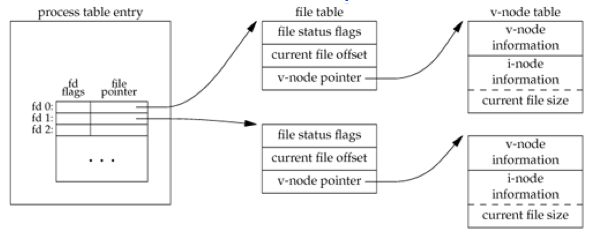
\includegraphics[scale=0.8,angle=-90]{pics/open-files.eps} \\
\end{center}

\subsection{File Sharing}
Knowing this, here's what happens with each of the calls we discussed earlier:

\begin{itemize}
	\item after each {\tt write} completes, the current file offset in the
		file table entry is incremented.  (If current\_file\_offset $>$
		current\_file\_size, change current file size in i-node table entry.)
	\item If file was opened {\tt O\_APPEND} set corresponding flag in file status
		flags in file table. For each {\tt write}, current file offset is first set to
		current file size from the i-node entry.
	\item {\tt lseek} simply adjusts current file offset in file table entry
	\item to {\tt lseek} to the end of a file, just copy current file size into
		current file offset.
\end{itemize}

\subsection{File Sharing}
\begin{center}
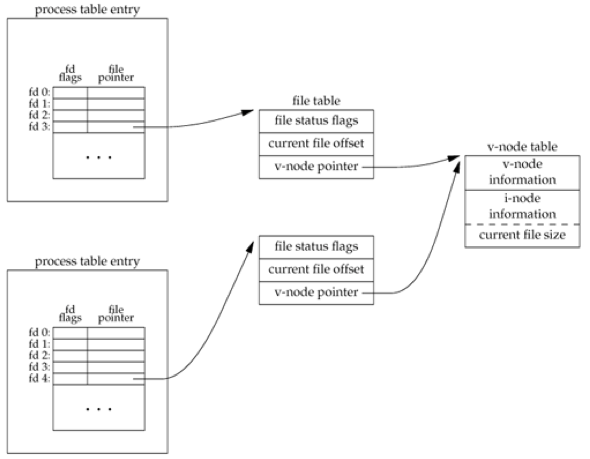
\includegraphics[scale=0.8,angle=-90]{pics/open-files-sharing.eps} \\
\end{center}


\subsection{Atomic Operations}

In order to ensure consistency across multiple writes, we require {\em
atomicity} in some operations.
\\

An operation is atomic if either {\em all} of the steps are performed or
{\em none} of the steps are performed.
\\

Suppose UNIX didn't have {\tt O\_APPEND} (early versions didn't). To
append, you'd have to do this:
\\

\small
\begin{verbatim}
if (lseek(fd, 0L, 2) < 0) {        /* position to EOF */
    fprintf(stderr, "lseek error\n");
    exit(1);
}

if (write(fd, buff, 100) != 100) { /* ...and write */
    fprintf(stderr, "write error\n");
    exit(1);
}
\end{verbatim}

\Normalsize

What if another process was doing the same thing to the same file?

\subsection{{\tt dup(2)} and {\tt dup2(2)}}
\small
\setlength{\unitlength}{1mm}
\begin{center}
	\begin{picture}(150,30)
		\thinlines
		\put(0,0){\framebox(130,30){}}
		\put(10,25){{\tt \#include <unistd.h>}}
		\put(10,17){{\tt int dup(int {\em oldd});}}
		\put(10,12){{\tt int dup2(int {\em oldd}, int {\em newd});}}
		\put(55,3){Both return new file descriptor if OK, -1 on error}
	\end{picture}
\end{center}
\Normalsize

An existing file descriptor can be duplicated with {\tt dup(2)} or duplicated to
a particular file descriptor value with {\tt dup2(2)}. As with {\tt open(2)}, {\tt
dup(2)} returns the lowest numbered unused file descriptor.
\\

Note the difference in scope of the file {\em descriptor} flags and the
file {\em status} flags compared to distinct processes.
\begin{center}
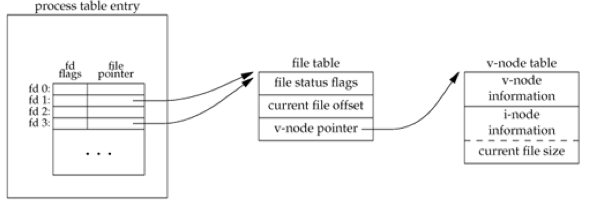
\includegraphics[scale=0.7,angle=-90]{pics/dup.eps} \\
\end{center}


\subsection{{\tt fcntl(2)}}
\small
\setlength{\unitlength}{1mm}
\begin{center}
	\begin{picture}(200,35)
		\thinlines
		\put(0,0){\framebox(180,35){}}
		\put(10,30){{\tt \#include <sys/types.h>}}
		\put(10,25){{\tt \#include <unistd.h>}}
		\put(10,20){{\tt \#include <fcntl.h>}}
		\put(10,12){{\tt int fcntl(int {\em filedes}, int {\em cmd}, ... /* int {\em arg} */);}}
		\put(110,3){Returns: depend on {\em cmd} if OK, -1 on error}
	\end{picture}
\end{center}
\Normalsize

{\tt fcntl(2)} is on of those "catch-all" functions with a myriad of purposes.
Here, they all relate to changing properties of an already open file. It can:
\vspace{.25in}

\begin{tabular}{l l l}
	{\bf cmd} & {\bf effect} & {\bf return value} \\
	\hline
	{\tt F\_DUPFD} & duplicate {\em filedes} (\small {\tt FD\_CLOEXEC} file descriptor flag is cleared )\Normalsize& new filedes \\
	{\tt F\_GETFD} & get the file descriptor flags for {\em filedes} & descriptor flags \\
	{\tt F\_SETFD} & set the file descriptor flags to the value of the third argument & not -1 \\
	{\tt F\_GETFL} & get the file status flags & status flags \\
	{\tt F\_SETFL} & set the file status flags & not -1
\end{tabular}
\vspace{.25in}

...as well as several other functions.

\subsection{{\tt fcntl(2)}}
\begin{verbatim}
$ dd if=/dev/urandom of=file bs=512 count=1024000
$ cc -Wall sync-cat.c -o scat
$ sed -e 's/\(.*O_SYNC.*\)/\/\/\1/' sync-cat.c > async-cat.c
$ cc -Wall async-cat.c -o ascat
$ time ./scat <file >out

$ time ./ascat <file >out

$

\end{verbatim}

\subsection{{\tt ioctl(2)}}
\small
\setlength{\unitlength}{1mm}
\begin{center}
	\begin{picture}(150,30)
		\thinlines
		\put(0,0){\framebox(130,30){}}
		\put(10,25){{\tt \#include <unistd.h>		/* SVR4 */}}
		\put(10,20){{\tt \#include <sys/ioctl.h>	/* 4.3+BSD */}}
		\put(10,12){{\tt int ioctl(int {\em filedes}, int {\em request}, ...);}}
		\put(55,3){Returns: -1 on error, something else if OK}
	\end{picture}
\end{center}
\Normalsize

Another catch-all function, this one is designed to handle device specifics
that can't be specified via any of the previous function calls. For example,
terminal I/O, magtape access, socket I/O, etc.

\subsection{Homework}
\begin{itemize}
	\item Reading:
		\begin{itemize}
			\item manual pages for the functions covered
			\item Stevens Chap. 3
		\end{itemize}
	\item Thinking:
		\begin{itemize}
			\item Stevens \# 3.5 (bourne shell syntax ``$>\&$'')
		\end{itemize}
	\item Coding:
		\begin{itemize}
			\item required: {\tt tcp(1)} (see website)
			\item extra credit: {\tt tcpm(1)} (see website)
		\end{itemize}
\end{itemize}

\end{document}
